\documentclass[12pt,letterpaper]{article}

\usepackage[utf8]{inputenc}

% Page layout
%\usepackage[a4paper]{geometry}
%\geometry{hscale=0.75,vscale=0.75,centering}
\usepackage{fullpage}

% Include images
\usepackage{graphicx}

% Math equations
\usepackage{amsmath}
\usepackage{amssymb}
\usepackage[french]{babel}

% Include Matlab code with accents
\usepackage{listingsutf8}
\lstset{inputencoding=utf8/latin1}
\usepackage[framed]{mcode}


\begin{document}

    \begin{titlepage}
    \vspace*{3.5cm}
    \begin{center} 
        \LARGE{ \textbf{INF6800 - Conception geométrique assistée par ordinateur} }\\[1cm]
        \Large{Travail pratique numéro 1.}\\
        \normalsize{05/02/2014}\\[1cm]
        \normalsize{ \textit{Anis Benyoub} }
    	\begin{figure}[ht]
	\centering
	\end{figure}
    \end{center}
    
\end{titlepage}
     
	\newpage
	
    \section{Infos:}
	J'ai rendu les fichiers ainsi que le makefile mais pas les fichiers de projet visual studio.

    \section{Bases et Courbes B-Spline:}
	\setlength{\parindent}{1cm}

	Dans cette partie j'ai implémenté le calcul d'une courbe B-Spline. Pour faire cela il faut itérer sur le vecteur nodal de manière uniforme. Dans notre cas, le domaine est toujours entre 0 et 1. Normalement c'est entre U[0] et U[size(U)].\\

	Pour chacune des valeurs de u calculées, on évalue les bases b-spline de manière iterative.\\

	Pour ce j'ai utilisé les algorithmes proposés dans le NURBS BOOK. On determine l'intervalle des noeuds concernés puis on évalue les fonctions de base (dont on se sert ensuite pour évaluer la valeur de la courbe au paramètre u).\\
	
	Dans le cas ou le degrés et le nombre de points sont égaux on retombe sur le cas des courbes de bezier.\\
	Voici le resultat visuel que donne cette partie:
\begin{figure}[h!]
	\centering
	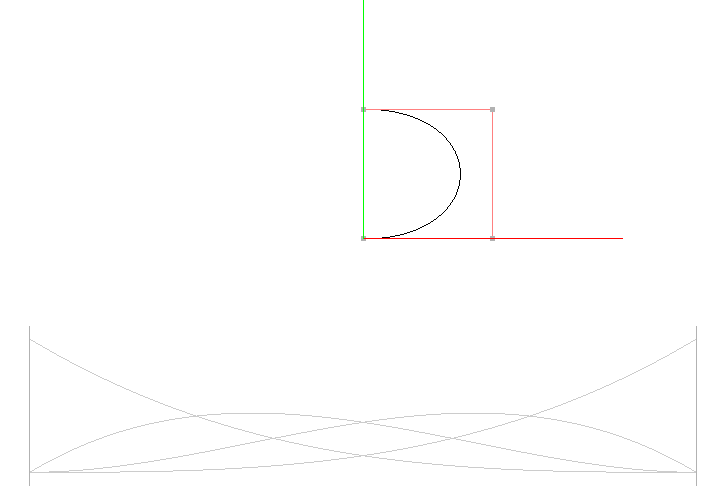
\includegraphics[scale=0.3]{images/img1.png}
	\caption{\textit{Rendu de la scene pour n == p == 4}}
\end{figure}
	
	Dans le cas ou on augmente le nombre de points tout en gardant le même ordre, nous ne sommes plus dans le cas des courbes b-spline.\\\\
	Voici le resultat visuel que donne cette partie:
	\newpage
\begin{figure}[h!]
	\centering
	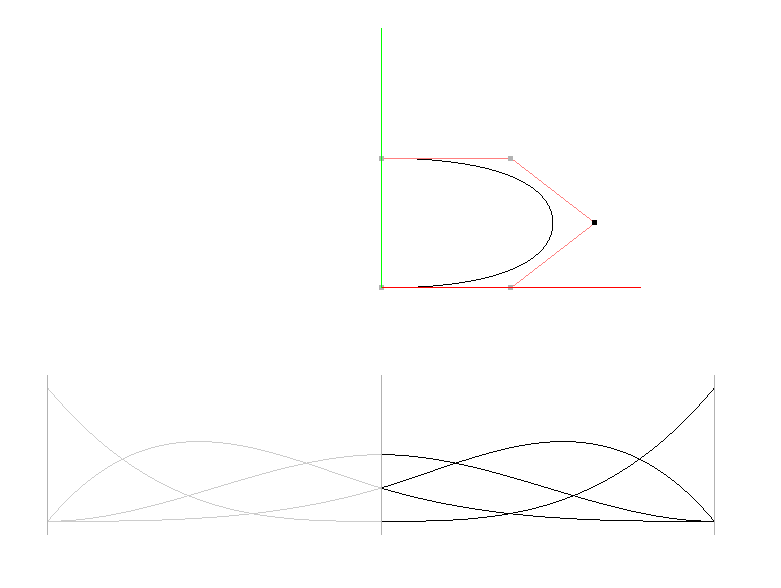
\includegraphics[scale=0.3]{images/img2.png}
	\caption{\textit{Rendu de la scene pour n == 5 et p == 4}}
\end{figure}
\section{Surfaces B-Spline:}
	\setlength{\parindent}{1cm}
	Dans la même optique que celle des courbes, j'ai implémenté le calcul d'une surface b-spline. Il faut effectuer le même calcul que pour la courbe, mais dans chacune des directions cette fois ci. On va donc échantilloner sur dans les deux intervalles correspondant aux deux vecteurs nodaux.\\
	
	On va donc calculer les dérivées partielles de chacun des points. J'ai utilisé les implémentation proposée par le NURBS BOOK de la même manière que pour les courbes la logique es très similaire.\\
	
	La normale est calculée en se basant sur les deux dérivée partielles de la courbe au point (u,v) courant.\\
	\newpage
	Voici le resultat visuel que donne cette partie:
\begin{figure}[h!]
	\centering
	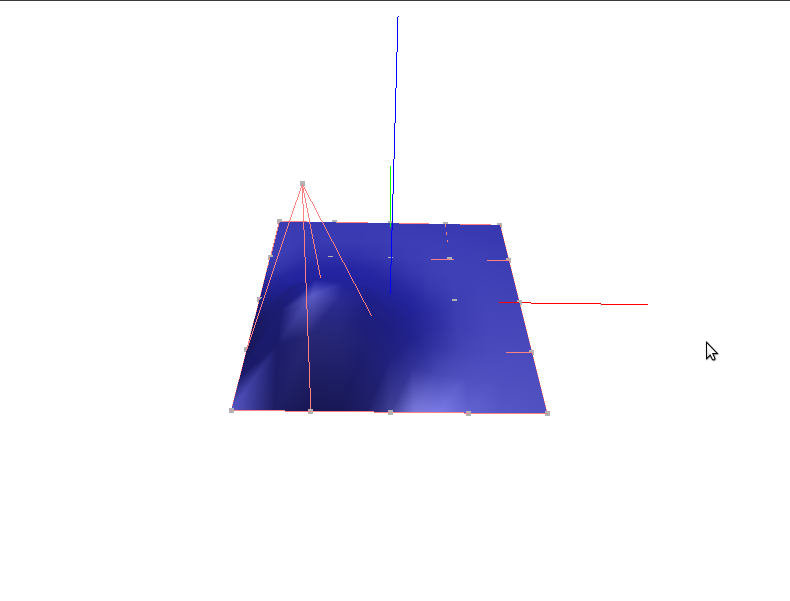
\includegraphics[scale=0.3]{images/img3.png}
	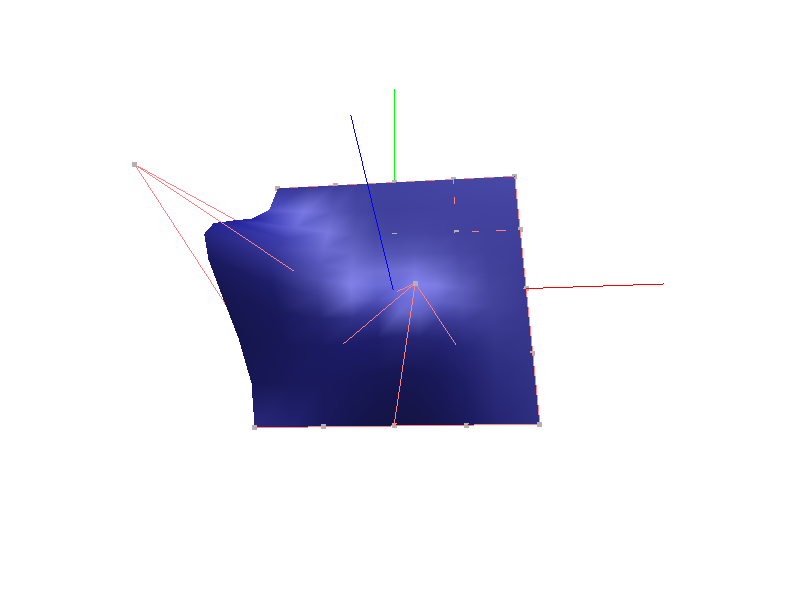
\includegraphics[scale=0.3]{images/img4.png}
	\caption{\textit{Deformation du plan et de ses normales à l'aide des surfaces b-splines}}
\end{figure}

\end{document}

